\subsection{Display Interfaces}

\begin{frame}{Display panels refreshing}
  \begin{itemize}
  \item Most display panel technologies need frequent pixel updates: \textbf{refreshing}
    \begin{itemize}
    \item Colors would fade out without refresh
    \item Panels usually lack internal memory to self-refresh
    \end{itemize}
  \item Requires a \textbf{fixed refresh rate}:
    \begin{itemize}
    \item Capped by the display technology or display interface
    \item Directly impacts smoothness: minimum is usually \(30~Hz\)
    \item The whole frame must be sent over each time
    \end{itemize}
  \item Requires \textbf{synchronization points}:
    \begin{itemize}
    \item Vertical: beginning of a new frame
    \item Horizontal: beginning of a new line
    \end{itemize}
  \item Requires \textbf{blank times}:
    \begin{itemize}
    \item Account for line/frame preparation time
    \item Initially for CRT electron gun repositioning
    \item More or less useful depending on the technology
    \end{itemize}
  \end{itemize}
\end{frame}

\begin{frame}{Display timings and modes}
  \begin{itemize}
  \item Timings coordinate how a frame is \textbf{transmitted to a display over time}
  \item Required signals are synced to a \textbf{pixel clock} (time base)
  \item Display timings are split in a few stages (horizontal and vertical):
    \begin{enumerate}
    \item Sync pulse (vsync/hsync)
    \item Back porch (vbp/hbp): blanking
    \item Active region (vactive/hactive)
    \item Front porch (vfp/hfp): blanking
    \end{enumerate}
  \item Pixels are transmitted during the \textbf{horizontal active region} (one line)
  \item A \textbf{display mode} groups all timing and signal characterization information
    \begin{itemize}
    \item Signals are \textbf{generated by the CRTC} according to the display mode
    \end{itemize}
  \item Monitors usually support \textbf{multiple modes} (and dimensions):
    \begin{itemize}
    \item Standard modes are defined by VESA
    \item Extra specific modes for the monitor can be supported
    \end{itemize}
  \end{itemize}
\end{frame}

\begin{frame}{Display timings and modes (illustrated)}
  \begin{center}
  \includegraphics[width=0.8\textwidth]{slides/graphics-hardware-display-interfaces/display-timings.pdf}
  \end{center}

  \begin{itemize}
  \item The unit for horizontal stages is \textbf{one pixel clock period}
  \item The unit for vertical stages is \textbf{one line's duration}
  \end{itemize}
\end{frame}

\begin{frame}{Display timings and modes (panel example)}

  \begin{minipage}[b]{0.35\textwidth}
    \centering
    \vspace{2em}
    \includegraphics[width=\textwidth]{slides/graphics-hardware-display-interfaces/timings-table.png}
    \textit{\small AT070TN94 panel datasheet}
    \vfill~
  \end{minipage}
  \hfill
  \begin{minipage}[b]{0.6\textwidth}
    \small
    \begin{itemize}
    \item \(hsync = thpw = 20 \in \llbracket 1;40 \rrbracket\)\\
    \(hbp = thb - thpw = 46 - 20 = 26\) (from diagram)\\
    \(hactive = thd = 800\)\\
    \(hfp = thfp = 210 \in \llbracket 16;354 \rrbracket\)\\
    \(htotal = hsync + hbp + hactive + hfp = 1056\)

    \item \(vsync = tvpw = 10 \in \llbracket 1;20 \rrbracket\)\\
    \(vbp = tvb - tvpw = 23 - 10 = 13\) (from diagram)\\
    \(vactive = tvd = 480\)\\
    \(vfp = tvfp = 22 \in \llbracket 7;147 \rrbracket\)\\
    \(vtotal = vsync + vbp + vactive + vfp = 525\)
    \item 1 frame takes: \(vtotal \times htotal = 554400~t_{clk}\)\\
    60 frames take: \(vtotal \times htotal \times 60 = 33264000~t_{clk}\)\\
    60 fps requires: \(f_{clk} \geq 33.264~MHz\)
    \end{itemize}
  \end{minipage}
  \vspace{0.5em}

  \begin{itemize}
  \item Panels usually support a \textbf{range of timings}
  \item The pixel clock rate is often \textbf{rounded} (refresh rate not always strictly respected)
  \end{itemize}

\end{frame}

\begin{frame}{Side-channel and identification}
  \begin{itemize}
  \item Monitor display connectors often come with a \textbf{Display Data Channel} (DDC)
    \begin{itemize}
    \item Side-bus to allow communication between host and display
    \item Usually based on I2C, quite slow (\(\approx 100~kHz\))
    \end{itemize}
  \item DDC provides access to the \textbf{Extended Display Identification Data} (EDID)
    \begin{itemize}
    \item Contains the list of supported modes in a standard format
    \item Usually stored in an EEPROM at I2C address \(0x50\)
    \end{itemize}
  \item Another common monitor signal is \textbf{Hotplug Detect} (HPD)
    \begin{itemize}
    \item Connected to a pin of the connector, asserted with a cable plugged
    \item Can be wired to an interrupt pin to detect connection changes
    \end{itemize}
  \item Direct panel interfaces (not monitors) usually lack DDC, EDID and HPD
    \begin{itemize}
      \item Panel is always considered connected
      \item Modes need to be known in advance
    \end{itemize}
  \end{itemize}
\end{frame}

\begin{frame}{Extra display interface features and EDID extensions}
  \begin{itemize}
  \item The EDID standard keeps evolving and exposes new features through extensions
  \item Configuration data for each feature is embedded in the EDID
  \item More or fewer features are supported depending on the display interface
  \item Common extra display interface features:
    \begin{itemize}
    \item \textbf{Interlaced}: Every other pixel line is sent at a time, alternating between top-fields and bottom-fields; Allows faster refreshing for CRTs, needs deinterlacing for progressive panels;
    \item \textbf{Audio}: Send audio in addition to pixels, during blanking periods;
    \item \textbf{Stereoscopy}: Pixel data is split between two screens that show a different geometrical perspective, providing 3D perception;
    \item \textbf{Variable Refresh Rate} (VRR): Pixel data can be sent at any point and does not need to conform to a given refresh rate;
    \item \textbf{Consumer Electronic Control} (CEC): Remote control features on a dedicated bus;
    \item \textbf{High-Bandwidth Digital Content Protection} (HDCP): Anti-copy protection
    \end{itemize}
  \end{itemize}
\end{frame}

\begin{frame}{Types of display interfaces}
  \begin{itemize}
  \item Legacy display interfaces are usually \textbf{analog}:
  \begin{itemize}
    \item Transmission through a DAC-based chain
    \item Lack of precision, noise and chain error: not pixel-perfect, capped
    \item Requires few signal pins (1 per color channel and sync or less)
  \end{itemize}
  \item Recent interfaces are usually \textbf{digital}:
    \begin{itemize}
    \item Encoded binary transmission, usually with dedicated clock
    \item Encoders contain a controller (logic) and a PHY (signal)
    \item Pixel data is expected to be bit-perfect \textit{(but noise still exists)}
    \end{itemize}
  \item Digital interfaces can be \textbf{parallelized}:
    \begin{itemize}
    \item One signal per color bit (e.g. 24 signals for 24-bit RGB), clock and sync
    \item One clock cycle for one pixel (low clock rate)
    \end{itemize}
  \item Or they can be \textbf{serialized}:
    \begin{itemize}
    \item Pixel data is sent over physical lanes (one or more)
    \item One clock cycle for one bit on each lane (high clock rate)
    \end{itemize}
  \end{itemize}
\end{frame}

\begin{frame}{Types of display interfaces (illustrated)}
  \begin{center}
    \includegraphics[width=0.7\textwidth]{slides/graphics-hardware-display-interfaces/display-interface-encoders.pdf}
  \end{center}
\end{frame}

\begin{frame}{VGA display interface}
  \begin{itemize}
  \item \textbf{Video Graphics Array} (VGA), since 1987 (IBM)
    \begin{itemize}
    \item \textbf{Analog} pixel data on 3 pins (R-G-B), DAC encoder to \(0.7~V\) peak-to-peak
    \item \textbf{Per-channel pixel streaming} (voltage change), following mode timings
    \item \textbf{Hsync} and \textbf{vsync} signals, I2C SDA and SDL \textbf{DDC} signals
    \item Hotplug detection with R/G/B pins \textbf{current sensing}
    \item Using a DB-15 connector for signals:
    \end{itemize}
  \begin{center}
    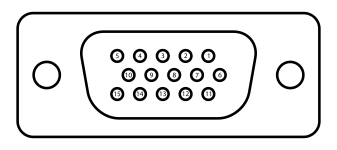
\includegraphics[height=2em]{slides/graphics-hardware-display-interfaces/vga-pinout.pdf}
  \end{center}
  \begin{itemize}
  \item \textbf{Pixel}: Red, Green, Blue {\footnotesize(1, 2, 3)}, Ground returns {\footnotesize(6, 7, 8)}
  \item \textbf{Sync}: Hsync, Vsync {\footnotesize(13, 14)}
  \item \textbf{Side}: DDC SDA, DDC SCL {\footnotesize(12, 15)}
  \item \textbf{Power}: \(+5~V\) {\footnotesize(9)}, Ground {\footnotesize(10)}
  \end{itemize}
  \end{itemize}

\end{frame}

\begin{frame}{VGA display interface (illustrated)}
  \begin{center}
    \includegraphics[width=\textwidth]{slides/graphics-hardware-display-interfaces/a13-olinuxino-vga.png}
  \end{center}

  \begin{itemize}
  \item Very basic VGA encoder from parallel signals, DDC excluded
  \item Resistor ladder for digital-to-analog conversion\\
  \textit{using SN74ALVC244 voltage level shifters (\(1.8~V\) to \(3.3~V\)), clamping diodes}
  \item 6 most-significant bits only, 2 least-significant bits set to 0\\
  \textit{D0-D1, D8-D9 and D16-D17 are not routed}
  \end{itemize}
\end{frame}

\begin{frame}{DVI display interface}
  \begin{itemize}
  \item \textbf{Digital Visual Interface} (DVI), since 1999 (DDWG)
    \begin{itemize}
    \item \textbf{DVI-A}: Analog only, comparable to VGA
    \item \textbf{DVI-D}: Digital only, single-link (3 data lanes) or dual-link (6 data lanes)
    \item \textbf{DVI-I}: Both analog and digital supported, single-link or dual-link
    \item Digital serial link using \textbf{Transition-Minimized Differential Signaling} (TMDS)
    \item Dedicated \textbf{DDC} and \textbf{HPD} signals
    \item Using a subset or variation of the full \textbf{DVI-I connector} for signals:
    \end{itemize}
  \begin{center}
    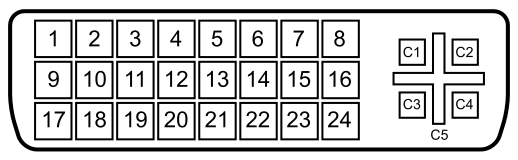
\includegraphics[height=2em]{slides/graphics-hardware-display-interfaces/dvi-pinout.pdf}
  \end{center}
  \begin{itemize}
  \item \textbf{TMDS}: Data+ {\footnotesize(2, 5, 10, 13, 18, 21)}, Data- {\footnotesize(1, 4, 9, 12, 17, 20)}, Clock {\footnotesize(23, 24)}
  \item \textbf{Analog pixel}: Red, Green, Blue {\footnotesize(C1, C2, C3)}, Ground {\footnotesize(C5)}
  \item \textbf{Analog sync}: Hsync, Vsync {\footnotesize(C4, 8)}
  \item \textbf{Side}: DDC SDA, DDC SCL {\footnotesize(7, 6)}, HPD {\footnotesize(16)}
  \item \textbf{Power}: \(+5~V\) {\footnotesize(14)}, Ground {\footnotesize(15)}
  \end{itemize}
  \end{itemize}
\end{frame}

\begin{frame}{HDMI display interface}
  \begin{itemize}
  \item \textbf{High-Definition Multimedia Interface} (HDMI), since 2002 (HDMI Forum)
    \begin{itemize}
    \item Similar to \textbf{DVI-D}: no analog, 3 TMDS data lanes (R-G-B)
    \item Adding the use of AVI infoframes for meta-data and audio
    \item \textbf{High bandwidth} \((\leq 48~Gbit/s)\) (2.1) and clock speeds \((\leq 340~MHz)\)
    \item \textbf{Extra features}: Audio, CEC (1.2), HDR (1.3), 4K (1.4), Stereoscopy (1.4),\\8K-10K (2.1), DSC (2.1), HFR (\(120~Hz\)), per-frame HDR (2.1)
    \item Using a dedicated (and proprietary) \textbf{HDMI connector} for signals:
    \end{itemize}
  \begin{center}
    \includegraphics[height=2em]{slides/graphics-hardware-display-interfaces/hdmi-pinout.pdf}
  \end{center}
  \begin{itemize}
  \item \textbf{TMDS}: Data+ {\footnotesize(1, 4, 7)}, Data- {\footnotesize(3, 6, 9)}, Clock {\footnotesize(10, 12)}
  \item \textbf{Side}: SDA, SCL {\footnotesize(16, 15)}, HPD {\footnotesize(19)}, CEC {\footnotesize(13)}
  \item \textbf{Power}: \(+5~V\) {\footnotesize(18)}, Ground {\footnotesize(17)}
  \end{itemize}
  \end{itemize}
\end{frame}

\begin{frame}{DP/eDP display interface}
  \begin{itemize}
  \item \textbf{DisplayPort} (DP), since 2008 (VESA)
    \begin{itemize}
    \item Digital serial link with 4 data lanes using \textbf{Low-Voltage Differential Signaling} (LVDS)
    or TMDS for DP Dual-Mode (DP++), compatible with DVI-D and HDMI
    \item Using \textbf{packets} for video/audio data and meta-data 
    \item Auxiliary channel encapsulating I2C DDC, CEC and more (e.g. USB)
    \item \textbf{High bandwidth} \((\leq 77.37~Gbit/s)\) (2.0)
    \item \textbf{Extra features}: Audio, CEC, HDR (1.4), 4K (1.3), Stereoscopy (1.2),\\8K (1.3-1.4),  10K-16K (2.0)
    \item \textbf{Multi-Stream Transport} (MST) to chain displays
    \item Using a dedicated (and proprietary) \textbf{DisplayPort connector} for signals:
    \end{itemize}
  \begin{center}
    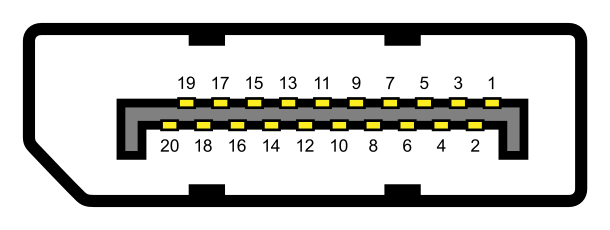
\includegraphics[height=2em]{slides/graphics-hardware-display-interfaces/dp-pinout.pdf}
  \end{center}
  \begin{itemize}
  \item \textbf{LVDS/TMDS}: ML+ {\footnotesize(1, 4, 7, 10)}, ML- {\footnotesize(3, 6, 9, 12)}
  \item \textbf{Side}: AUX+ (15), AUX- (17), HPD (18)
  \item \textbf{Power}: \(+3.3~V\) {\footnotesize(20)}, Ground {\footnotesize(2, 5, 8, 11, 16)}
  \end{itemize}
  \item \textbf{Embedded DisplayPort} (eDP) for internal panels (without connector)
  \end{itemize}
\end{frame}

\begin{frame}{LVDS and DSI display interfaces}

% TODO split and add photo of custom LVDS connector as well as a DSI panel (librem 5 dvt?)

  \begin{itemize}
  \item \textbf{Low Voltage Differential Signaling} (LVDS)
    \begin{itemize}
    \item Generic digital serial link with clock and data signals (3-4 lanes) using LVDS
    \item Pixel data and control (vsync, hsync, display enable) sent as bits on lanes
    \item Uses a fixed mode, no DDC, no packets
    \item Specified with the JEIDA, LDI, DSIM and VESA specifications
    \item For internal panels, exposed with specific connectors
    \item Common for laptop panels
    \end{itemize}
  \end{itemize}
  \begin{itemize}
  \item \textbf{Display Serial Interface} (DSI), since 2006 (MIPI)
    \begin{itemize}
    \item Digital serial link with clock and up to 4 data lanes using LVDS
    \item Using \textbf{packets} for video data and meta-data
    \item Commands for configuration can be issued with the \textbf{DSI Command Set} (DCS)\\
    \textit{Generic base with proprietary vendor-specific extensions}
    \item For internal panels, exposed with specific connectors
    \item Common for mobile devices' panels
    \end{itemize}
  \end{itemize}
\end{frame}

\begin{frame}{DPI display interface}
  \begin{itemize}
  \item \textbf{Display Parallel Interface} (DPI)
    \begin{itemize}
    \item Generic parallel digital interface, with 1 signal per color bit, clock and sync
    \item Exists with different numbers of bits: 24 (8-8-8), 18 (6-6-6) or 16 (5-6-5)\\
    \textit{Dithering is required when using 16 or 18 bits}
    \item Sends pixel data bits following mode timings
    \item Base signals: color data bits, vsync, hsync
    \item Extra signals: display enable (DE)
    \item Beware: sync and DE signals can be active-high or active-low
    \item For internal panels, requires many signals
    \end{itemize}
  \end{itemize}
\end{frame}

\begin{frame}{Bridges/transcoders}
  \begin{itemize}
  \item Not every display interface is supported by the hardware at hand
  \item Bridges or transcoders are used to translate from one interface to another
  \item They are composed of a decoder and an encoder (in a single package)
  \item Usually standalone and transparent, often only replicate timings\\
  \textit{but some can have a side-bus for configuration and fine-tuning}
  \item Example: VGA interfaces are usually bridged from digital interfaces nowadays
  \end{itemize}

  \begin{center}
  \includegraphics[height=6em]{slides/graphics-hardware-display-interfaces/dp-dvi-bridge.jpg}\\
  \textit{\small A DP to DVI bridge}
  \end{center}
\end{frame}
